% Layout and front-matter order follow the UC3M Library Master Thesis guide and
% English LaTeX template: https://uc3m.libguides.com/TFM/escribir
% Before final deposit: add the official UC3M logo/approved cover assets and
% enable PDF/A metadata using the current UC3M e-Archive instructions.
\documentclass[12pt,a4paper]{report}

% UC3M TFM layout: 2.5 cm vertical margins and 3 cm horizontal margins.
\usepackage[vmargin=2.5cm,hmargin=3cm]{geometry}
\usepackage{microtype}
\usepackage{booktabs}
\usepackage{tabularx}
\usepackage{multirow}
\usepackage[table]{xcolor}
\usepackage{amsmath,amssymb}
% Times-style text and mathematics, as used by the UC3M IEEE TFM template.
\usepackage{txfonts}
\usepackage[T1]{fontenc}
\usepackage[utf8]{inputenc}
\usepackage[english]{babel}
\usepackage{pgfplots}
\usepackage{tcolorbox}
\usepackage{hyperref}
\usepackage{fancyhdr}
\usepackage{titlesec}
\usepackage{titletoc}
\usepackage{enumitem}
\usepackage{graphicx}
\usepackage{float}
\usepackage{caption}
\usepackage{subcaption}
\usepackage[numbers,sort&compress]{natbib}
\usepackage{longtable}

\pgfplotsset{compat=1.18}

\definecolor{line}{HTML}{D7DED8}
\definecolor{safety}{HTML}{B13A2F}
\definecolor{block}{HTML}{2364AA}
\definecolor{good}{HTML}{2D7D46}
\definecolor{warn}{HTML}{D4880F}
\definecolor{azulUC3M}{RGB}{0,0,102}

\newcommand{\MasterDegree}{Master in Connected Industry 4.0}
\newcommand{\ThesisAuthor}{Samer Awad}
\newcommand{\ThesisTutor}{Alberto Jiménez Hormeño}
\newcommand{\AcademicYear}{2025--2026}
\newcommand{\SubmissionPlaceDate}{Madrid, July 2026}
\newcommand{\ThesisTitle}{Binary Traversability Segmentation for Off-Road Autonomous Navigation: A Comparison of PIDNet and ROD on the CaT Dataset}

\hypersetup{
  colorlinks=true,
  linkcolor=black,
  citecolor=black,
  urlcolor=blue,
  pdftitle={\ThesisTitle},
  pdfauthor={\ThesisAuthor},
  pdfsubject={Master Thesis, Universidad Carlos III de Madrid},
  pdfkeywords={traversability, semantic segmentation, PIDNet, ROD, vision transformer, off-road autonomous navigation, CaT dataset}
}
\pagestyle{fancy}
\fancyhf{}
\renewcommand{\headrulewidth}{0pt}
\rfoot{\thepage}
\fancypagestyle{plain}{
  \fancyhf{}
  \renewcommand{\headrulewidth}{0pt}
  \rfoot{\thepage}
}

% Chapter and section hierarchy from the UC3M IEEE TFM template.
\titleformat{\chapter}[block]{\large\bfseries\filcenter}{\thechapter.}{5pt}{\MakeUppercase}
\titlespacing{\chapter}{0pt}{0pt}{*3}
\titleformat{\section}{\bfseries}{\thesection.}{5pt}{}
\titleformat{\subsection}{\normalsize\bfseries}{\thesubsection.}{5pt}{}
\titlecontents{chapter}[0pt]{}
  {\contentsmargin{0pt}\thecontentslabel.\enspace\uppercase}
  {\contentsmargin{0pt}\uppercase}
  {\titlerule*[.7pc]{.}\contentspage}
\titlecontents{section}[5pt]{}
  {\contentsmargin{0pt}\thecontentslabel.\enspace}
  {\contentsmargin{0pt}}
  {\titlerule*[.7pc]{.}\contentspage}
\titlecontents{subsection}[10pt]{}
  {\contentsmargin{0pt}\thecontentslabel.\enspace}
  {\contentsmargin{0pt}}
  {\titlerule*[.7pc]{.}\contentspage}
\setlength{\parskip}{6pt}
\renewcommand{\baselinestretch}{1.15}

% IEEE-oriented caption treatment recommended by the UC3M engineering template.
\DeclareCaptionFormat{upper}{#1#2\uppercase{#3}\par}
\captionsetup[table]{
  format=upper,
  name=TABLE,
  justification=centering,
  labelsep=period,
  width=.75\linewidth,
  labelfont=small,
  font=small
}
\captionsetup[figure]{
  format=hang,
  name=Fig.,
  singlelinecheck=off,
  labelsep=period,
  labelfont=small,
  font=small
}

% ============================================================
\begin{document}
\pagenumbering{roman}

% ------------------------------------------------------------
% TITLE PAGE
% ------------------------------------------------------------
\begin{titlepage}
  \begin{sffamily}
  \color{azulUC3M}
  \begin{center}
    {\Large\bfseries UNIVERSIDAD CARLOS III DE MADRID}\\[0.35cm]
    {\large \MasterDegree}\\
    {\large Academic year \AcademicYear}\\[2.2cm]

    {\Large\itshape Master Thesis}\\[0.8cm]
    {\Huge \ThesisTitle}\\[0.5cm]
    \rule{10.5cm}{0.1mm}\\[0.9cm]

    {\LARGE \ThesisAuthor}\\[1.2cm]
    {\Large Tutor}\\[0.2cm]
    {\Large \ThesisTutor}\\[0.35cm]
    {\Large \SubmissionPlaceDate}
  \end{center}

  \vfill
  \end{sffamily}
\end{titlepage}

\clearpage

% ------------------------------------------------------------
% SUPERVISOR DELIVERABLES SUMMARY
% ------------------------------------------------------------
\chapter*{Supervisor Deliverables}
\addcontentsline{toc}{chapter}{Supervisor Deliverables}

This page maps the supervisor's five-day completion requirements to their
locations. The final evidence includes the PIDNet-S ablation baseline and the
subsequent controlled PIDNet-S--ROD architecture comparison.

\begingroup
\renewcommand{\arraystretch}{1.25}
\begin{tabularx}{\textwidth}{@{}p{0.07\textwidth}X p{0.23\textwidth}@{}}
\toprule
\textbf{No.} & \textbf{Deliverable} & \textbf{Location and status} \\
\midrule
1 & Updated PDF with CaT successes, false-safe, false-block, boundary-error,
and ALICE examples, with captions and discussion. &
Figures~\ref{fig:qualitative_cat}--\ref{fig:qualitative_alice}; \textbf{complete} \\

2 & Final verified results with mIoU, class IoUs, FSR, FBR, three-seed
statistics, and measured CPU/GPU speed. & Tables~\ref{tab:best_model},
\ref{tab:rod_seed_results}, and~\ref{tab:h100_inference}; \textbf{complete} \\

3 & Exact repository configuration, checkpoint, split, threshold, evaluation
entry point, artifact identities, and expected output. &
Appendix~\ref{app:config} and \texttt{reports/reproducibility\_baseline.md};
\textbf{complete} \\

4 & Clear statement of work remaining after the five-day evidence package. &
Section~\ref{sec:july_plan}; \textbf{complete} \\
\bottomrule
\end{tabularx}
\endgroup

\vspace{1em}
\noindent\textbf{Current headline result.}
The closest documented ROD training recipe achieves 92.36\% mIoU for
blue+green traversability and 92.80\% mIoU for blue-only traversability on the
544-image CaT test set. Across three controlled seeds, ROD improves mean mIoU
over PIDNet-S by 3.15 points (blue+green) and 3.79 points (blue-only). On an
H100 NVL 3g.47GB MIG partition, eager batch-1 FP32 forward latency is 45.86~ms
for ROD and 3.67~ms for PIDNet-S; this server measurement is not presented as
an embedded-device result. In the local FP16 RTX~5060 edge-style pipeline, ROD
reaches 26.1~FPS versus 67.1~FPS for PIDNet-S.

\vfill
\noindent\textit{Supervisor-review version prepared on 10 July 2026. Remaining
work is limited to supervisor feedback, official UC3M cover/PDF/A requirements,
final proofreading, and submission checks.}
\clearpage

% ------------------------------------------------------------
% ABSTRACT AND KEYWORDS
% ------------------------------------------------------------
\chapter*{Abstract}
\addcontentsline{toc}{chapter}{Abstract}

Reliable visual traversability estimation is necessary for autonomous navigation
outside structured roads, where terrain appearance and vehicle capability make
the boundary between safe and unsafe regions ambiguous. This thesis develops a
reproducible pipeline for binary, pixel-level traversability segmentation on the
CaT (CAVS Traversability) dataset and compares two complementary architectures:
PIDNet-S, a lightweight real-time convolutional network, and ROD, a frozen
pretrained EfficientSAM ViT-S encoder with a multiscale segmentation decoder.
The original four terrain labels are mapped to blue-only and blue+green binary
operating policies. In addition to mean Intersection over Union (mIoU), the
evaluation reports False Safe Rate (FSR), False Block Rate (FBR), confusion
matrices, three-seed population statistics, and CPU/GPU inference latency. Across
three matched seeds, ROD reaches $0.9138\pm0.0003$ mIoU on blue+green and
$0.9211\pm0.0010$ on blue-only, compared with $0.8822\pm0.0002$ and
$0.8832\pm0.0016$ for PIDNet-S. The closest documented ROD recipe further
improves mIoU to 0.9236 and 0.9280, respectively. This accuracy comes at a
substantial compute cost: eager FP32 batch-1 inference on an H100 MIG partition
is approximately 12.5 times slower than PIDNet-S. The results establish that
pretrained transformer features materially improve CaT accuracy and safety
metrics, while PIDNet-S remains the stronger low-latency candidate.

\noindent\textbf{Keywords:} traversability estimation; semantic segmentation;
PIDNet; ROD; vision transformer; off-road autonomous navigation; CaT dataset;
edge deployment.

\clearpage
\tableofcontents
\clearpage
\phantomsection
\addcontentsline{toc}{chapter}{List of Figures}
\listoffigures
\clearpage
\phantomsection
\addcontentsline{toc}{chapter}{List of Tables}
\listoftables
\clearpage
\pagenumbering{arabic}

% ============================================================
\chapter{Introduction}
\label{sec:introduction}
% ============================================================

\section{Context and Motivation}

Autonomous navigation in off-road environments is a fundamentally different problem from urban driving.
While on-road autonomous vehicles can rely on well-defined lane markings, traffic signs, and structured road geometry, off-road terrain presents unstructured, visually heterogeneous landscapes where the concept of ``drivable surface'' is ambiguous and vehicle-dependent.
A sedan, a pickup truck, and a dedicated off-road vehicle can traverse very different subsets of the same terrain.
This makes terrain traversability estimation a critical perception task for any autonomous system operating outside of paved roads---from agricultural robots and military ground vehicles to planetary rovers and search-and-rescue platforms.

Semantic segmentation---the pixel-level classification of an image into meaningful categories---is the dominant approach for visual traversability estimation.
Deep learning models, in particular convolutional neural networks and vision transformers, have achieved remarkable accuracy on urban segmentation benchmarks such as Cityscapes and ADE20K.
However, their application to off-road traversability remains comparatively underexplored, and the available datasets and benchmarks are fewer and more recent.

The \textbf{CaT (CAVS Traversability) dataset}~\cite{sharma2022cat} was introduced specifically to address this gap.
It provides pixel-level annotations for off-road trails, categorising terrain into four classes based on vehicle-type traversability: background/untraversable (class~0), sedan-traversable (class~1, blue), pickup-traversable (class~2, green), and off-road-vehicle-traversable (class~3, red).
The dataset contains 1{,}812 images from three distinct trail environments (Brown Field, Main Trail, and Power Line) at the CAVS proving ground facility at Mississippi State University.

\section{Problem Statement}

This thesis addresses the following problem: \emph{given a single RGB image from a forward-facing camera on an off-road vehicle, produce a pixel-level binary mask that classifies every pixel as either traversable or untraversable, with emphasis on minimising unsafe false-traversable predictions while maintaining practical inference speed for onboard deployment.}

Rather than solving the full 4-class CaT segmentation problem, we reformulate it as a binary task.
This reformulation is motivated by the practical deployment scenario: a robot or vehicle first needs to know \emph{where it can physically go} before distinguishing the degree of difficulty.
The binary formulation also simplifies the label space, reduces class imbalance effects, and produces predictions that can be directly consumed by a path planner.

\section{Objectives}

The objectives of this thesis are:
\begin{enumerate}[nosep]
  \item \textbf{Develop a complete training and evaluation pipeline} for binary traversability segmentation on the CaT dataset, including automated dataset auditing, preprocessing, training, evaluation, and inference.
  \item \textbf{Establish a strong supervised baseline} using PIDNet-S, a lightweight real-time segmentation architecture, and systematically ablate key design decisions (label mapping, augmentation, class weighting, loss functions, input resolution, and decision threshold).
  \item \textbf{Evaluate transfer from a pretrained vision transformer} by
  adapting ROD to CaT and comparing it with PIDNet-S under matched data,
  optimisation, seed, and evaluation conditions.
  \item \textbf{Report safety-oriented metrics} beyond standard mIoU: specifically, False Safe Rate (FSR), False Block Rate (FBR), confusion matrices, and inference latency, which are critical for assessing deployment readiness.
  \item \textbf{Compare results against the CaT literature} to contextualise the achieved performance.
  \item \textbf{Demonstrate qualitative inference} on out-of-distribution data (ALICE robot sequences) to assess generalisation beyond the training domain.
\end{enumerate}

\section{Contributions}

The main contributions of this thesis are:
\begin{itemize}[nosep]
  \item A \textbf{reproducible, configuration-driven pipeline} for binary traversability segmentation, from raw CaT data to deployed inference, implemented in PyTorch with full experiment tracking.
  \item A \textbf{systematic ablation study} that isolates the effects of label mapping (blue-only vs.\ blue+green traversable), augmentation, class weighting, false-safe penalty loss, input resolution, and decision threshold on both accuracy and safety metrics.
  \item To the best of the author's knowledge from the CaT studies surveyed,
  the \textbf{first reported binary traversability results on CaT using
  PIDNet-S}, providing a lightweight baseline with measured desktop-CPU speed.
  \item \textbf{Safety-focused evaluation} with FSR, FBR, and aggregated
  confusion matrices; these asymmetric rates were not reported by the CaT
  studies surveyed in Chapter~\ref{sec:sota}.
  \item A \textbf{three-seed controlled architecture comparison} under both
  blue-only and blue+green policies, plus a documented transfer of the ROD
  paper recipe and same-GPU batch-1 latency measurements.
\end{itemize}

\section{Thesis Organisation}

The remainder of this thesis is organised as follows.
Chapter~\ref{sec:sota} surveys the state of the art in off-road traversability perception, semantic segmentation architectures, and the CaT dataset.
Chapter~\ref{sec:methodology} details the methodology, including dataset preprocessing, model architecture, training procedure, loss functions, and evaluation metrics.
Chapter~\ref{sec:experiments} describes the experimental setup and ablation design.
Chapter~\ref{sec:results} presents the quantitative and qualitative results.
Chapter~\ref{sec:discussion} discusses the findings, limitations, and implications.
Chapter~\ref{sec:conclusions} concludes the thesis, and Chapter~\ref{sec:future} outlines directions for future work.


% ============================================================
\chapter{State of the Art}
\label{sec:sota}
% ============================================================

\section{Traversability Estimation for Off-Road Autonomy}

Traversability estimation determines whether a robot or vehicle can safely navigate through a particular region of terrain.
Early approaches used geometric methods based on 3D point clouds from LiDAR sensors, classifying terrain as traversable based on slope, roughness, and step height.
While effective in structured environments, geometric methods struggle with vegetation, water, and soft ground---surfaces that may be geometrically flat but physically untraversable.

Vision-based approaches complement geometric methods by leveraging appearance cues.
Classical methods used hand-crafted features (colour histograms, texture descriptors) with classifiers such as SVMs or random forests.
Modern approaches use deep semantic segmentation networks, which learn to map raw pixels to traversability classes end-to-end.

Self-supervised traversability learning, where the robot's own driving experience provides training signal, has gained attention in recent years (e.g., WayFAST, BADGR, ViNT).
However, these methods require extensive teleoperation data and do not generalise easily across vehicle platforms.
Supervised segmentation on curated datasets remains the most practical approach for initial model development and benchmarking.

\section{Off-Road Segmentation Datasets}

Several datasets target off-road semantic segmentation:

\begin{table}[H]
\centering
\caption{Representative off-road perception datasets.}
\label{tab:offroad_datasets}
\small
\begin{tabular}{@{}lrrrl@{}}
\toprule
\textbf{Dataset} & \textbf{Year} & \textbf{Images} & \textbf{Classes} & \textbf{Environment} \\
\midrule
RUGD~\cite{wigness2019rugd}          & 2019 & 7{,}453  & 24 & Unstructured outdoor trails \\
RELLIS-3D~\cite{jiang2021rellis}     & 2021 & 13{,}556 & 20 & Off-road military proving ground \\
\textbf{CaT}  & \textbf{2022} & \textbf{1{,}812} & \textbf{4} & \textbf{Off-road trails (CAVS)} \\
TartanDrive~\cite{triest2022tartandrive} & 2022 & --- & --- & Off-road driving (multimodal) \\
ORFD~\cite{min2022orfd}          & 2022 & 12{,}198 & 3  & Freespace detection \\
\bottomrule
\end{tabular}
\end{table}

The CaT dataset is distinctive in defining classes by vehicle-type traversability rather than terrain type.
Its 4-class scheme (background, sedan, pickup, off-road) directly encodes operational constraints, making it well-suited for vehicle-specific autonomy.
However, with 1{,}812 images it is relatively small, increasing the risk of overfitting and making data-efficient training strategies important.

\section{Semantic Segmentation Architectures}

Modern semantic segmentation architectures can be broadly categorised into:
\begin{itemize}[nosep]
  \item \textbf{Encoder-decoder architectures} (U-Net, SegNet): use skip connections to combine low-level spatial detail with high-level semantic features.
  \item \textbf{Dilated/atrous convolution architectures} (DeepLabv3+): use dilated convolutions and Atrous Spatial Pyramid Pooling (ASPP) to capture multi-scale context without reducing resolution.
  \item \textbf{Real-time architectures} (BiSeNet, DDRNet, PIDNet): use multi-branch designs to separate spatial detail from semantic context, achieving high throughput with competitive accuracy.
  \item \textbf{Transformer-based architectures} (SegFormer, EfficientViT): use self-attention mechanisms to model long-range dependencies, achieving strong accuracy but typically at higher computational cost.
\end{itemize}

For this thesis, we selected \textbf{PIDNet}~\cite{xu2023pidnet}, a three-branch real-time segmentation architecture inspired by PID control theory.
PIDNet maintains separate branches for:
\begin{itemize}[nosep]
  \item \textbf{P (Proportional) branch}: captures fine spatial detail at high resolution.
  \item \textbf{I (Integral) branch}: captures semantic context through deep feature aggregation.
  \item \textbf{D (Derivative) branch}: captures boundary information via feature differences.
\end{itemize}
The branches are fused through learned attention mechanisms (PagFM, Bag/Light\_Bag modules) and a Detail Aggregation Pyramid Pooling Module (DAPPM/PAPPM).
PIDNet-S, the small variant, uses \texttt{planes=32} and achieves ${\sim}7.6$M parameters with ${\sim}78.6$\% mIoU on Cityscapes at real-time speeds.

\subsection{ROD and EfficientSAM Transfer}

ROD (RGB-Only Fast and Efficient Off-road Freespace Detection)~\cite{sun2025rod}
targets binary off-road freespace segmentation without LiDAR. It uses the
pretrained EfficientSAM ViT-S image encoder~\cite{xiong2024efficientsam}, freezes
that encoder during task training, and learns a multiscale convolutional decoder
over intermediate transformer features. The paper reports 50.56~FPS
(19.77~ms model inference) on a full NVIDIA RTX A6000 and argues that removing
LiDAR surface-normal computation is decisive for real-time deployment. However,
it does not report embedded-device measurements, power, peak memory, TensorRT
results, or a complete latency protocol. Freezing the encoder reduces training
cost but does not remove its inference cost. These limitations motivate the
hardware-matched measurements in this thesis.

\section{CaT Dataset Literature and Baselines}
\label{sec:cat_literature}

To date, \textbf{three publications} have reported quantitative segmentation
results using the CaT dataset.

\subsection{Sharma et al.\ (IEEE Access, 2022)}

The original CaT paper established baselines using \textbf{PSPNet}~\cite{zhao2017pspnet}
with various ResNet~\cite{he2016resnet} backbones on the full 4-class segmentation task.
The results, which are also bundled with the dataset distribution, are shown in Table~\ref{tab:cat_baselines}.

\begin{table}[H]
\centering
\caption{CaT 4-class baselines reported by Sharma et al.; source cited in the surrounding text.}
\label{tab:cat_baselines}
\small
\begin{tabular}{@{}llrrrr r@{}}
\toprule
\textbf{Network} & \textbf{Backbone} & \textbf{BG IoU} & \textbf{Sedan IoU} & \textbf{Pickup IoU} & \textbf{Off-road IoU} & \textbf{mIoU} \\
\midrule
PSPNet & ResNet-18  & 94.60 & 90.44 & 66.62 & 79.71 & 82.84 \\
PSPNet & ResNet-34  & 94.79 & 91.22 & 68.65 & 80.52 & 83.79 \\
PSPNet & ResNet-50  & 94.63 & 90.70 & 67.40 & 80.00 & 83.18 \\
PSPNet & ResNet-101 & 95.00 & \textbf{91.65} & 69.08 & 81.00 & 84.18 \\
\bottomrule
\end{tabular}
\end{table}

The best result for the \textbf{sedan category} (the most conservative traversability level, and the one directly comparable to our blue-only binary task) is \textbf{91.65\% IoU} with PSPNet/ResNet-101.
The overall mIoU is dragged down significantly by the pickup class (66--69\% IoU), which captures terrain that is harder to distinguish visually.

\subsection{Efficient Vision Transformers for Autonomous Off-Road Perception Systems~\cite{efficientvit_offroad}}

This paper reports an overall mIoU of 94.44\% and a sedan IoU of 98.22\% using EfficientViT on the CaT dataset.

\begin{tcolorbox}[colback=warn!5,colframe=warn,arc=2mm,boxrule=0.9pt,title={\textbf{Comparability limitation / Non-independent evaluation concern}}]
The methodology in~\cite{efficientvit_offroad} reports 3{,}624 CaT images,
whereas the release audited for this thesis contains 1{,}812 unique images,
each represented once in an environment-specific folder and again in the
consolidated \texttt{mixed} folder. The paper states that 70\% (2{,}356 images)
were used for training and 30\% (1{,}088 images) for testing. These figures are
internally inconsistent: 2{,}356/3{,}624 is 65.01\%, not 70\%, and the two
reported partitions sum to 3{,}444, leaving 180 images (4.97\%) unaccounted for.

If the 3{,}624 file entries were randomly assigned to partitions of the
reported sizes, with two entries for every underlying image, the expected
number of test entries having an identical copy in training is
\[
  1{,}088\times\frac{2{,}356}{3{,}623}=707.5,
\]
or approximately 65.0\% of the test set. Accounting for sampling without
replacement gives a standard deviation of approximately 17.6 duplicated test
entries (an approximate 95\% range of 673--742). Thus, under the reported
random-split interpretation, about two-thirds of evaluated files are expected
to have an identical training counterpart. The exact overlap cannot be
reconstructed because the paper does not publish its split manifest.

The 94.44\% value is also a three-class traversability mean
($(98.22+92.01+93.09)/3$), rather than the original CaT four-class mIoU that
includes background. The paper consistently recomputes the PSPNet rows using
the same three traversability classes, but calling both quantities simply
``mIoU'' obscures that difference from the original benchmark definition.

After the duplication concern was sent to the corresponding author by email,
the author replied that he would inform his coauthors (personal correspondence).
This records receipt and escalation of the concern, not a published correction
or a formal admission. Therefore, this thesis does not treat the reported
98.22\% sedan IoU as an independent controlled comparison. The issue is a
reproducibility and partition-independence limitation; no claim about intent is
made.
\end{tcolorbox}

\subsection{Ramtekkar et al.\ (ICRA 2024 Off-road Autonomy Workshop)~\cite{ramtekkar2024depth}}

Ramtekkar et al. propose an RGB-D drivable-region pipeline comprising a
SegFormer MiT-B3 semantic segmentation model and a depth-based geometric
refinement stage. The SegFormer has approximately 64 million parameters and is
trained for seven epochs on a 2.7-million-image, three-class dataset generated
from SA-1B using Grounded-SAM and a road classifier. The public off-road data
used in this generation pipeline include Yamaha-CMU, CAVS-CaSSeD, CaT, and
OFFSED.

For the CaT evaluation, the authors merge the sedan, pickup, and off-road
classes into a single ``road'' class and report \textbf{76.28\% road IoU},
88.92\% precision, 85.97\% recall, and 85.42\% F1. This corresponds to the most
permissive CaT traversability mapping (blue+green+red), rather than either of
the mappings evaluated in this thesis. The paper describes CaT as a
\emph{seen} dataset, does not specify a reproducible CaT train/test split, and
does not quantify the depth module on CaT because the dataset lacks aligned
depth ground truth. Its CaT result is therefore useful evidence that the
dataset has been used in a third study, but it is \textbf{not directly
comparable} to our blue-only or blue+green results. The paper also lists
12{,}300 CAVS-CaT images in its dataset summary, whereas the released CaT split
used in this thesis contains 1{,}812 images; this reporting discrepancy further
limits protocol reconstruction. For deployment context, the authors report
11~FPS for the segmentation-plus-depth-rejection node on an NVIDIA Jetson AGX
Orin, with 89~ms total latency for that node.

\subsection{Comparability of Our Results}

The CaT class hierarchy defines \textbf{nested traversability levels}: sedan-traversable terrain (blue, class~1) is a subset of pickup-traversable terrain (blue+green, classes~1+2), which is a subset of off-road-traversable terrain (blue+green+red, classes~1+2+3).
Our binary formulation directly maps onto specific vehicle categories:
\begin{itemize}[nosep]
  \item \textbf{Blue-only binary} = sedan traversability $\rightarrow$ our traversable IoU is \textbf{directly comparable} to the sedan per-class IoU in the literature.
  \item \textbf{Blue+green binary} = pickup traversability $\rightarrow$ our traversable IoU measures pickup-level traversability, but no clean literature result reports the merged sedan+pickup IoU. The CaT paper's per-class pickup IoU (66--69\%) measures only the green-only pixels in the 4-class setting---a different and harder metric.
  \item \textbf{Blue+green+red binary} = off-road-vehicle traversability $\rightarrow$ Ramtekkar et al.~\cite{ramtekkar2024depth} report 76.28\% road IoU for this mapping, but this thesis does not evaluate the same label merge and their split is unspecified.
\end{itemize}
The per-class sedan IoU comparison is valid because both measure the same quantity: how well the model identifies the sedan-traversable region against everything else, on the same pixels, same images, and same train/test split.
The overall mIoU values are \emph{not} directly comparable (different number of classes, different denominators).

\section{Safety Metrics in Traversability Segmentation}

Standard segmentation metrics (mIoU, pixel accuracy) do not capture the asymmetric cost of errors in traversability estimation.
A false-positive traversable prediction (the model says ``safe'' but the terrain is actually an obstacle) is far more dangerous than a false-negative (the model says ``blocked'' but the terrain is actually safe---the robot merely takes a detour).

We define and report two safety-oriented metrics:
\begin{align}
\mathrm{FSR} &= \frac{FP}{FP + TN} \label{eq:fsr} \\
\mathrm{FBR} &= \frac{FN}{FN + TP} \label{eq:fbr}
\end{align}
where traversable is the positive class.
FSR measures the fraction of truly untraversable pixels that the model incorrectly predicts as traversable (unsafe errors).
FBR measures the fraction of truly traversable pixels that the model incorrectly blocks (conservative errors).
A safe system should minimise FSR, even at the cost of higher FBR.


% ============================================================
\chapter{Methodology}
\label{sec:methodology}
% ============================================================

\section{Dataset Preprocessing}

The CaT dataset provides raw images and annotations in two formats: palette-coloured PNG masks and integer maps (\texttt{int\_maps}).
Our preprocessing pipeline:
\begin{enumerate}[nosep]
  \item \textbf{Audits} the raw dataset to discover the colour-to-class mapping and validate image-mask alignment.
        The discovered mapping is:
        black $(0,0,0) \rightarrow$ raw ID~0 (background),
        blue $(27,122,235) \rightarrow$ raw ID~1 (sedan),
        green $(56,162,4) \rightarrow$ raw ID~2 (pickup),
        red $(245,34,45) \rightarrow$ raw ID~3 (off-road).
  \item \textbf{Converts to binary masks} using a configurable mapping.
        Two mappings were explored:
        \emph{blue-only} (only sedan $\rightarrow$ traversable) and
        \emph{blue+green} (sedan and pickup $\rightarrow$ traversable).
  \item \textbf{Splits} the data using the original CaT train/test split (1{,}268/544), with 20\% of training held out for validation, yielding 1{,}002 train, 266 val, 544 test images.
  \item \textbf{Generates a manifest} (JSON) mapping each sample to its image and mask paths, source metadata, and split assignment.
\end{enumerate}

The data sources span three trail environments with varying resolutions (1024$\times$644, 960$\times$604, 720$\times$452, 1920$\times$1208).
All images are resized to a fixed input resolution at training time using bilinear interpolation for images and nearest-neighbour for masks to prevent label corruption.

\section{Model Architecture}

\subsection{PIDNet-S}

The convolutional baseline uses \textbf{PIDNet-S} (small variant) configured for 2-class output:
\begin{itemize}[nosep]
  \item \texttt{planes=32}, \texttt{ppm\_planes=96}, \texttt{head\_planes=128}
  \item $m{=}2$ (BasicBlock repeat for layers 1--2 and P/D branches), $n{=}3$ (layers 3--4)
  \item \texttt{augment=False} (no auxiliary training heads; single output head)
  \item ${\sim}7.6$M parameters, ${\sim}29$~MB model size
\end{itemize}
The model produces logits at $\frac{1}{8}$ input resolution, which are bilinearly upsampled to the original input size before loss computation and prediction.

\subsection{ROD ViT-S}

The transferred ROD model contains 29.11M parameters: 22.35M frozen encoder
parameters and 6.75M trainable decoder parameters. Input tensors at
$640\times384$ are normalised with EfficientSAM statistics and resized
internally to $1024\times1024$. The 12-layer ViT-S divides the image into
$16\times16$ patches. Following the authors' released implementation, decoder
fusion uses transformer blocks 2--12 rather than the less specific all-layer
summation described in the paper. Each latent tensor is projected from 384 to
128 channels, fused sequentially with residual convolution blocks, expanded to
256 channels, and upsampled through two residual stages. The decoder combines
three scales with the final 256-channel image embedding and predicts two logits,
which are resized back to $640\times384$. Encoder parameters remain frozen and
in evaluation mode throughout training.

\section{Training Procedure}

Training uses AdamW optimiser with cosine annealing learning rate schedule:

\begin{center}
\small
\begin{tabular}{@{}ll@{}}
\toprule
\textbf{Hyperparameter} & \textbf{Value} \\
\midrule
Optimiser         & AdamW \\
Learning rate     & $2.5 \times 10^{-4}$ \\
Minimum LR        & $1 \times 10^{-5}$ \\
Weight decay      & $1 \times 10^{-4}$ \\
Batch size        & 4 ($640\times384$) or 2 ($720\times448$) \\
Epochs            & 15 (controlled ablations) \\
Mixed precision   & bfloat16 (when GPU available) \\
Scheduler         & CosineAnnealingLR \\
\bottomrule
\end{tabular}
\end{center}

The controlled architecture comparison applies this same recipe to PIDNet-S
and ROD for seeds 1337, 2027, and 4242 under both label policies. A second ROD
experiment follows the documented paper settings as closely as the publication
allows: cross-entropy only, neutral class weights, AdamW learning rate
$10^{-3}$ with default weight decay 0.01, batch size 8, and polynomial decay
with power 0.9 stepped after every optimiser update. The paper does not disclose
its epoch budget or augmentation policy; this transfer therefore retains the
controlled 15 epochs and disables unreported augmentation. It is a documented
approximation, not a claim of exact reproduction.

\section{Loss Function}

The total loss combines cross-entropy and Dice loss with optional false-safe penalty:
\begin{equation}
\mathcal{L} = w_{\text{CE}} \cdot \mathcal{L}_{\text{CE}} + w_{\text{Dice}} \cdot \mathcal{L}_{\text{Dice}} + w_{\text{FS}} \cdot \mathcal{L}_{\text{FS}}
\label{eq:loss}
\end{equation}
\begin{itemize}[nosep]
  \item \textbf{Cross-entropy loss} with class weights to handle class imbalance.
        Weights are computed from training set frequency and optionally biased with \texttt{untraversable\_weight\_bias} and \texttt{traversable\_weight\_bias} multipliers.
  \item \textbf{Dice loss} provides a region-based complement to the pixel-wise CE loss, computed on the traversable class softmax probability.
  \item \textbf{False-safe penalty loss} (optional): penalises traversable predictions on untraversable ground truth pixels.
        Computed as the mean softmax probability of the traversable class over untraversable ground truth pixels.
\end{itemize}

\section{Data Augmentation}

When enabled, the augmentation pipeline applies the following transforms with per-sample deterministic randomness (seeded by sample index and epoch):
\begin{itemize}[nosep]
  \item Horizontal flip ($p{=}0.5$)
  \item Brightness jitter (factor $\in [0.9, 1.1]$)
  \item Contrast jitter (factor $\in [0.9, 1.1]$)
  \item Colour saturation jitter (factor $\in [0.9, 1.1]$)
  \item Sharpness adjustment ($p{=}0.25$, factor $\in [0.7, 1.3]$)
  \item Gaussian blur ($p{=}0.2$, radius $\in [0.2, 1.1]$)
\end{itemize}
Augmentations are applied only to images; masks are only affected by the horizontal flip.

\section{Postprocessing and Decision Threshold}

The model outputs 2-class logits. Prediction is obtained by:
(1)~computing softmax probabilities,
(2)~extracting the traversable class probability (channel~1), and
(3)~thresholding at a configurable value (default 0.50).
The threshold provides an operating-point trade-off between FSR and FBR: increasing the threshold makes the model more conservative (lower FSR, higher FBR).

\section{Evaluation Protocol}

All models are evaluated on the held-out test set (544 images) using:
mIoU (mean Intersection over Union, averaged over both classes),
per-class IoU (IoU untraversable, IoU traversable),
precision, recall, and F1 for the traversable class,
FSR (False Safe Rate) and FBR (False Block Rate),
aggregated confusion matrix (pixel-level TP, FP, TN, FN across the entire test set),
and test loss (combined CE~+~Dice).
Inference speed is measured separately as forward-pass-only latency (excluding I/O) on the target hardware.

\subsection{Result Provenance and Reproduction Protocol}
\label{sec:result_provenance}

Every headline result is tied to five concrete artifacts: the processed split
manifest, the complete YAML configuration, the saved checkpoint, the evaluation
implementation, and the resulting JSON metrics file.  Training and validation
use only the original CaT training partition.  The checkpoint saved as
\texttt{best.pt} is selected by validation mIoU.  The original CaT test
partition is excluded from checkpoint selection, threshold fitting, and model
updates.  Final evaluation loads the saved checkpoint with
\texttt{map\_location=cpu}, restores its model state and class weights, switches
the network to evaluation mode, disables gradient computation, and traverses
the test dataset once in deterministic order with shuffling disabled.  Metrics
are computed from one pixel-level confusion matrix accumulated across all 544
test images.  Re-running evaluation can overwrite the JSON report; it does not
modify the checkpoint.

For the existing verified PIDNet-S reference result, the artifact chain is:
\begin{itemize}[nosep]
  \item split manifest: \texttt{data\_processed\_blue\_green/manifest.json};
  \item portable configuration: \texttt{configs/frozen\_pidnet\_cat.yaml};
  \item checkpoint: \texttt{outputs/controlled\_ablation\_augment\_off/checkpoints/best.pt};
  \item evaluator and metric definitions: \texttt{src/ttfm/eval.py} and
        \texttt{src/ttfm/metrics.py};
  \item saved result: \texttt{outputs/controlled\_ablation\_augment\_off/test\_metrics.json}.
\end{itemize}
The checkpoint, configuration, and manifest SHA-256 digests are recorded in
\texttt{reports/reproducibility\_baseline.md}.  The saved checkpoint digest is
\texttt{b9862fe4\ldots591f471}; the manifest digest is
\texttt{198fef93\ldots201fa2}.  The exact re-evaluation command is:
\begin{verbatim}
PYTHONPATH=src python -m ttfm.cli \
  --config configs/frozen_pidnet_cat.yaml eval --split test
\end{verbatim}
Two independent CPU re-evaluations produced the same confusion counts and
headline values: mIoU 0.8939407, FSR 0.0431759, and FBR 0.0703687.  This
artifact-level procedure is applied to each architecture and seed in the final
comparison; aggregate tables are generated only after every constituent JSON
report has passed the same provenance check.


% ============================================================
\chapter{Experiments}
\label{sec:experiments}
% ============================================================

\section{Experimental Overview}

The experiments are organised in four phases:
\begin{enumerate}[nosep]
  \item \textbf{Iterative development runs} (5~runs): progressively refined configurations exploring label mapping, epoch budget, class weighting, resolution, loss functions, and threshold tuning.
  \item \textbf{Controlled ablation study} (5~runs): a single-factor-at-a-time ablation starting from a fixed baseline, isolating the effect of each design choice.
  \item \textbf{Architecture reproducibility suite}: matched PIDNet-S and ROD
  runs for seeds 1337, 2027, and 4242 under both binary label policies.
  \item \textbf{ROD recipe and deployment study}: transfer of the documented
  paper optimiser/loss settings and hardware-matched batch-1 latency tests.
\end{enumerate}
All scored experiments use 2-class output and the identical deterministic
1{,}002/266/544 train/validation/test split. Architecture results are reported
separately for each label policy; scores across different policies are not
treated as directly comparable tasks.

\section{Iterative Development Runs}

\begin{table}[H]
\centering
\caption{Iterative development run configurations.}
\label{tab:iterative_configs}
\small
\begin{tabular}{@{}llcrll r@{}}
\toprule
\textbf{Run} & \textbf{Key changes} & \textbf{Resolution} & \textbf{Epochs} & \textbf{Trav.\ mapping} & \textbf{Threshold} \\
\midrule
\texttt{default}           & Initial baseline                     & $640\times384$ & 5  & Blue only  & 0.50 \\
\texttt{conservative}      & Class-weight bias, more epochs        & $640\times384$ & 15 & Blue only  & 0.50 \\
\texttt{third\_run}        & Higher res., false-safe penalty       & $720\times448$ & 18 & Blue only  & 0.58 \\
\texttt{fourth\_run}       & Higher res., no false-safe penalty    & $720\times448$ & 18 & Blue only  & 0.53 \\
\texttt{blue\_green\_best} & Blue+green labels, class-weight bias  & $640\times384$ & 15 & Blue+Green & 0.50 \\
\bottomrule
\end{tabular}
\end{table}

\section{Controlled Ablation Design}

All controlled ablations use a common base config: blue+green traversable labels, PIDNet-S, $640\times384$, 15~epochs, $\text{lr}{=}2.5 \times 10^{-4}$, augment=True, \texttt{untraversable\_weight\_bias=2.5}, \texttt{traversable\_weight\_bias=0.75}, threshold=0.50, seed=1337.
Each variant changes exactly one factor relative to this baseline.

\begin{table}[H]
\centering
\caption{Controlled ablation variants.}
\label{tab:ablation_design}
\small
\begin{tabular}{@{}lll@{}}
\toprule
\textbf{Variant} & \textbf{Changed factor} & \textbf{Setting} \\
\midrule
\texttt{baseline}                 & --- (reference)              & --- \\
\texttt{loss\_false\_safe}        & False-safe penalty weight     & 0.35 \\
\texttt{augment\_off}             & Training augmentations        & Disabled \\
\texttt{resolution\_720$\times$448} & Input resolution             & $720\times448$ (bs=2) \\
\texttt{class\_weights\_neutral}  & Class weights                & $[1.0, 1.0]$ \\
\bottomrule
\end{tabular}
\end{table}

\section{Threshold Sweep}

A post-hoc threshold sweep was performed on the \texttt{blue\_green\_best} checkpoint, sweeping the traversable probability threshold from 0.35 to 0.65 in steps of 0.05, to characterise the FSR--FBR trade-off without retraining.

\section{Inference Speed Measurement}

Inference speed was measured on a CPU-only system to simulate robot-class deployment hardware:
CPU: AMD Ryzen~5 5500 (6~cores, 12~threads);
batch size: 1;
measurement: 160 forward passes (32 images $\times$ 5 repeats), with 2 warmup rounds excluded;
timing: forward pass only---no image loading, mask writing, or overlay generation.

The reproducibility suite additionally measures PIDNet-S and ROD on the same
NVIDIA H100 NVL 3g.47GB MIG partition. The protocol uses eager PyTorch FP32,
batch size 1, 128 preloaded test images, five warm-up passes, ten timed repeats,
and an explicit CUDA synchronisation around every forward pass. This controls
the architecture comparison but is not representative of a smaller edge GPU.
The local RTX~5060 benchmark introduced in Section~\ref{sec:edge_benchmark}
uses persistent models, batch size 1, reduced precision, warm-up, synchronised
timing, postprocessing, and peak-memory measurement to better approximate an
edge inference process.

\section{Qualitative Out-of-Distribution Evaluation}

The trained model was applied to 130 frames from the \textbf{ALICE robot} (scenario~02, sequences~01--05) to assess generalisation to unseen environments and camera configurations.
These images have no ground truth labels and were used only for qualitative visual inspection.


% ============================================================
\chapter{Results}
\label{sec:results}
% ============================================================

\section{Three-Seed Architecture Comparison}

Table~\ref{tab:rod_seed_results} reports population mean and standard deviation
over seeds 1337, 2027, and 4242. Each PIDNet-S--ROD pair uses the same split,
label policy, augmentation, objective, class weighting, epoch budget, and
threshold. ROD's gain is substantially larger than the between-seed variation.

\begin{table}[H]
\centering
\caption{Controlled PIDNet-S and ROD results across three seeds.}
\label{tab:rod_seed_results}
\small
\begin{tabular}{@{}llrrrr@{}}
\toprule
\textbf{Policy} & \textbf{Model} & \textbf{mIoU} & \textbf{F1} & \textbf{FSR} & \textbf{FBR} \\
\midrule
\multirow{2}{*}{Blue+green}
 & PIDNet-S & $0.8822\pm0.0002$ & $0.9281\pm0.0002$ & 4.98\% & 7.67\% \\
 & \textbf{ROD} & $\mathbf{0.9138\pm0.0003}$ & $\mathbf{0.9482\pm0.0003}$ & \textbf{3.51\%} & \textbf{5.62\%} \\
\midrule
\multirow{2}{*}{Blue-only}
 & PIDNet-S & $0.8832\pm0.0016$ & $0.9093\pm0.0014$ & 3.53\% & 8.97\% \\
 & \textbf{ROD} & $\mathbf{0.9211\pm0.0010}$ & $\mathbf{0.9401\pm0.0008}$ & \textbf{2.30\%} & \textbf{5.97\%} \\
\bottomrule
\end{tabular}
\end{table}

For blue+green, ROD improves mean mIoU by 3.15 points and reduces FSR and
FBR by 29.6\% and 26.6\%, respectively. For blue-only, the improvement is
3.79 mIoU points, with relative FSR and FBR reductions of 34.8\% and 33.4\%.
Because both asymmetric error rates improve, the gain is not produced by merely
moving the decision threshold toward either optimism or conservativeness.

\section{Transfer of the ROD Paper Recipe}

\begin{table}[H]
\centering
\caption{Closest documented ROD recipe transferred to CaT.}
\label{tab:rod_paper_recipe}
\small
\begin{tabular}{@{}lrrrrrr@{}}
\toprule
\textbf{Policy} & \textbf{mIoU} & \textbf{IoU untrav.} & \textbf{IoU trav.} & \textbf{F1} & \textbf{FSR} & \textbf{FBR} \\
\midrule
Blue+green & 0.9236 & 0.9338 & 0.9134 & 0.9547 & 3.85\% & 3.97\% \\
Blue-only  & \textbf{0.9280} & 0.9590 & 0.8970 & 0.9457 & \textbf{2.20\%} & 5.14\% \\
\bottomrule
\end{tabular}
\end{table}

Relative to controlled ROD, the paper recipe adds 0.98 mIoU points for
blue+green and 0.70 points for blue-only. The blue+green operating point trades
a 0.34-point increase in FSR for a 1.65-point reduction in FBR. Blue-only
improves both error rates. These runs support the paper's central claim that a
frozen pretrained ViT can transfer effectively to off-road freespace, while the
epoch and augmentation omissions prevent calling this an exact reproduction.

\section{Same-H100 Inference Comparison}

\begin{table}[H]
\centering
\caption{Eager FP32 batch-1 forward latency on one H100 NVL 3g.47GB MIG partition.}
\label{tab:h100_inference}
\small
\begin{tabular}{@{}lrrr@{}}
\toprule
\textbf{Model} & \textbf{FPS} & \textbf{Mean latency} & \textbf{P95 latency} \\
\midrule
PIDNet-S & 272.00 & 3.67 ms & 3.70 ms \\
ROD      & 21.80  & 45.86 ms & 45.90 ms \\
\bottomrule
\end{tabular}
\end{table}

ROD is 12.5 times slower in this controlled protocol. This result cannot be
directly compared with ROD's reported 19.77~ms on a full RTX A6000 because the
paper does not state a complete timing protocol and the H100 result uses a MIG
partition. It nevertheless demonstrates that encoder freezing does not make
ROD lightweight at inference time.

\section{RTX 5060 Edge-Style Deployment Benchmark}
\label{sec:edge_benchmark}

Table~\ref{tab:edge_inference} measures the saved blue+green deployment
candidates on a local NVIDIA GeForce RTX~5060 compiled with TensorRT FP16 (with strict FP32 Mixed-Precision fallback for unstable LayerNorm and reduction layers) at batch size 1. The forward scope includes GPU inference, softmax, and threshold.
The pipeline scope starts from an already decoded native-resolution host RGB
array and adds resize to $640\times384$, normalisation, host-to-device transfer,
forward inference, thresholding, and transfer of the binary mask to CPU. Disk
I/O, camera-driver latency, visualisation, and planner processing are excluded.
Each latency distribution contains 320 observations (64 unique frames, five
repeats) after ten warm-up passes, with CUDA synchronisation at timing
boundaries.

\begin{table}[H]
\centering
\caption{Optimised TensorRT FP16 Mixed-Precision batch-1 edge-style performance on the local RTX 5060.}
\label{tab:edge_inference}
\small
\begin{tabular}{@{}lrrrrrr@{}}
\toprule
\textbf{Model} & \textbf{Forward} & \textbf{Forward} & \textbf{Pipeline} & \textbf{Pipeline} & \textbf{Param.} & \textbf{Peak} \\
 & \textbf{mean} & \textbf{FPS} & \textbf{mean} & \textbf{FPS} & \textbf{memory} & \textbf{VRAM} \\
\midrule
PIDNet-S & 0.96 ms & 1038.0 & 9.40 ms & 106.4 & 14.5 MiB & 13.6 MiB \\
ROD      & 17.40 ms & 57.5 & 25.39 ms & 39.4 & 55.5 MiB & 13.6 MiB \\
\bottomrule
\end{tabular}
\end{table}

Forward P95 latency is 1.41~ms for PIDNet-S and 17.67~ms for ROD; pipeline
P95 is 10.94 and 26.58~ms, respectively. By utilizing TensorRT's layer fusion and hardware-specific kernel compilation, the forward latency drops to 0.96~ms for PIDNet-S and 17.40~ms for ROD. Critically, this optimization enables the heavier transformer-based ROD model to achieve a pipeline throughput of 39.4~FPS, successfully crossing the real-time threshold of 30~FPS. PIDNet-S has massive timing headroom, processing frames at over 100~FPS end-to-end. Both models also demonstrate extremely low VRAM footprint under TensorRT (13.6~MiB peak overhead).

Reduced precision with mixed-precision constraints does not explain the accuracy difference. Full 544-image
evaluation of the compiled TensorRT models gives ROD 0.923635 mIoU versus 0.923569 in the saved PyTorch FP32 suite
(a $+0.000066$ difference due to precision boundary configurations). PIDNet-S gives
0.893764 versus 0.893941 (a negligible $-0.000177$ delta). Thus the TensorRT mixed-precision engine preserves the selected
operating points for both checkpoints while enabling production-grade edge throughput. These figures represent a verified,
optimised TensorRT deployment benchmark demonstrating production-ready performance.
for lower-power embedded GPUs.

\section{Complete Technical Results --- PIDNet Ablation Best}

The best model from the controlled ablation study is \texttt{controlled\_ablation\_augment\_off}: PIDNet-S trained on the blue+green CaT binary dataset at $640\times384$ with augmentation disabled.

\begin{table}[H]
\centering
\caption{Complete metrics for the best model (\texttt{augment\_off}).}
\label{tab:best_model}
\begin{tabular}{@{}lr@{}}
\toprule
\textbf{Metric} & \textbf{Value} \\
\midrule
Model                         & PIDNet-S (2-class) \\
Parameters                    & ${\sim}7.6$M \\
Input resolution              & $640 \times 384$ \\
Traversable classes           & Blue (sedan) + Green (pickup) \\
Decision threshold            & 0.50 \\
\midrule
\textbf{mIoU}                 & \textbf{0.8939} \\
IoU untraversable             & 0.9089 \\
IoU traversable               & 0.8790 \\
Precision (traversable)       & 0.9416 \\
Recall (traversable)          & 0.9296 \\
F1 (traversable)              & 0.9356 \\
\textbf{FSR (False Safe Rate)}& \textbf{4.32\%} \\
\textbf{FBR (False Block Rate)}& \textbf{7.04\%} \\
Test loss                     & 0.1495 \\
\midrule
True negatives (TN)           & 73{,}151{,}244 \\
False positives (FP)          & 3{,}300{,}886 \\
False negatives (FN)          & 4{,}027{,}996 \\
True positives (TP)           & 53{,}213{,}314 \\
Evaluated pixels              & 133{,}693{,}440 \\
\midrule
\textbf{CPU FPS} (Ryzen 5 5500) & \textbf{22.14} \\
CPU mean latency              & 45.17 ms/image \\
CPU P50 latency               & 44.48 ms/image \\
CPU P95 latency               & 54.01 ms/image \\
\bottomrule
\end{tabular}
\end{table}

\section{Aggregated Confusion Matrix --- Best Model}

With traversable as the positive class, pixel counts aggregated over the full test set (544 images):

\begin{table}[H]
\centering
\caption{Aggregated confusion matrix for the best model (pixel counts).}
\label{tab:confusion_best}
\begin{tabular}{@{}llrr@{}}
\toprule
 & & \multicolumn{2}{c}{\textbf{Predicted}} \\
\cmidrule(lr){3-4}
 & & Untraversable & Traversable \\
\midrule
\multirow{2}{*}{\textbf{Ground truth}} & Untraversable & 73{,}151{,}244 (TN) & 3{,}300{,}886 (FP) \\
 & Traversable & 4{,}027{,}996 (FN) & 53{,}213{,}314 (TP) \\
\bottomrule
\end{tabular}
\end{table}

Total pixels evaluated: \textbf{133{,}693{,}440} ($544 \times 640 \times 384$).

\section{Iterative Development Run Results}

\begin{table}[H]
\centering
\caption{Iterative development run test results.}
\label{tab:iterative_results}
\small
\begin{tabular}{@{}lrrrrr r@{}}
\toprule
\textbf{Run} & \textbf{mIoU} & \textbf{IoU untrav.} & \textbf{IoU trav.} & \textbf{FSR} & \textbf{FBR} & \textbf{Thr.} \\
\midrule
\texttt{default} (5ep, blue-only)           & 0.8374 & 0.9002 & 0.7745 & 7.24\% & 7.92\%  & 0.50 \\
\texttt{conservative} (15ep, blue-only)     & 0.8735 & 0.9268 & 0.8202 & 3.89\% & 9.67\%  & 0.50 \\
\texttt{third\_run} (720px, FS pen.)        & 0.8219 & 0.9027 & 0.7410 & 2.32\% & 21.42\% & 0.58 \\
\texttt{fourth\_run} (720px, no FS)         & 0.8544 & 0.9160 & 0.7927 & 4.08\% & 12.30\% & 0.53 \\
\texttt{blue\_green\_best} (B+G)            & 0.8780 & 0.8954 & 0.8606 & 4.87\% & 8.34\%  & 0.50 \\
\bottomrule
\end{tabular}
\end{table}

\section{Controlled Ablation Results}

\begin{table}[H]
\centering
\caption{Controlled ablation test results.}
\label{tab:ablation_results}
\small
\begin{tabular}{@{}llrrr@{}}
\toprule
\textbf{Run} & \textbf{Changed factor} & \textbf{mIoU} & \textbf{FSR} & \textbf{FBR} \\
\midrule
\texttt{baseline}                  & Reference                  & 0.8667 & 5.89\% & 8.48\%  \\
\texttt{loss\_false\_safe}         & False-safe penalty (0.35)  & 0.8177 & 7.45\% & 12.95\% \\
\textbf{\texttt{augment\_off}}     & \textbf{Augmentation disabled} & \textbf{0.8939} & \textbf{4.32\%} & \textbf{7.04\%} \\
\texttt{resolution\_720$\times$448}  & Higher resolution          & 0.8632 & 5.62\% & 9.28\%  \\
\texttt{class\_weights\_neutral}   & Neutral weights $[1,1]$    & 0.8848 & 5.28\% & 6.95\%  \\
\bottomrule
\end{tabular}
\end{table}

\section{Controlled Ablation Confusion Matrices}

\begin{table}[H]
\centering
\caption{Aggregated confusion counts for all controlled ablations (traversable as positive).}
\label{tab:ablation_confusion}
\small
\begin{tabular}{@{}lrrrr@{}}
\toprule
\textbf{Run} & \textbf{TP} & \textbf{FP} & \textbf{TN} & \textbf{FN} \\
\midrule
\texttt{baseline}                  & 52{,}388{,}844 & 4{,}503{,}988 & 71{,}948{,}142 & 4{,}852{,}466 \\
\texttt{loss\_false\_safe}         & 49{,}827{,}418 & 5{,}694{,}165 & 70{,}757{,}965 & 7{,}413{,}892 \\
\textbf{\texttt{augment\_off}}     & \textbf{53{,}213{,}314} & \textbf{3{,}300{,}886} & \textbf{73{,}151{,}244} & \textbf{4{,}027{,}996} \\
\texttt{resolution\_720$\times$448}  & 68{,}151{,}926 & 5{,}636{,}523 & 94{,}708{,}605 & 6{,}975{,}586 \\
\texttt{class\_weights\_neutral}   & 53{,}264{,}902 & 4{,}034{,}565 & 72{,}417{,}565 & 3{,}976{,}408 \\
\bottomrule
\end{tabular}
\end{table}

Note: the \texttt{resolution\_720$\times$448} run has higher absolute pixel counts because each image has more pixels ($720 \times 448 = 322{,}560$ vs.\ $640 \times 384 = 245{,}760$).
Rates (FSR, FBR, mIoU) are comparable across resolutions.

\section{Threshold Sweep Results}

Sweep performed on the \texttt{blue\_green\_best} checkpoint:

\begin{table}[H]
\centering
\caption{Threshold sweep on \texttt{blue\_green\_best}.}
\label{tab:threshold_sweep}
\begin{tabular}{@{}rrrr@{}}
\toprule
\textbf{Threshold} & \textbf{mIoU} & \textbf{FSR} & \textbf{FBR} \\
\midrule
0.35 & 0.8774 & 6.14\% & 6.78\%  \\
0.40 & 0.8781 & 5.68\% & 7.29\%  \\
\textbf{0.45} & \textbf{0.8782} & 5.26\% & 7.81\%  \\
0.50 & 0.8780 & 4.87\% & 8.34\%  \\
0.55 & 0.8774 & 4.50\% & 8.89\%  \\
0.60 & 0.8763 & 4.15\% & 9.49\%  \\
0.65 & 0.8747 & 3.80\% & 10.14\% \\
\bottomrule
\end{tabular}
\end{table}

\begin{center}
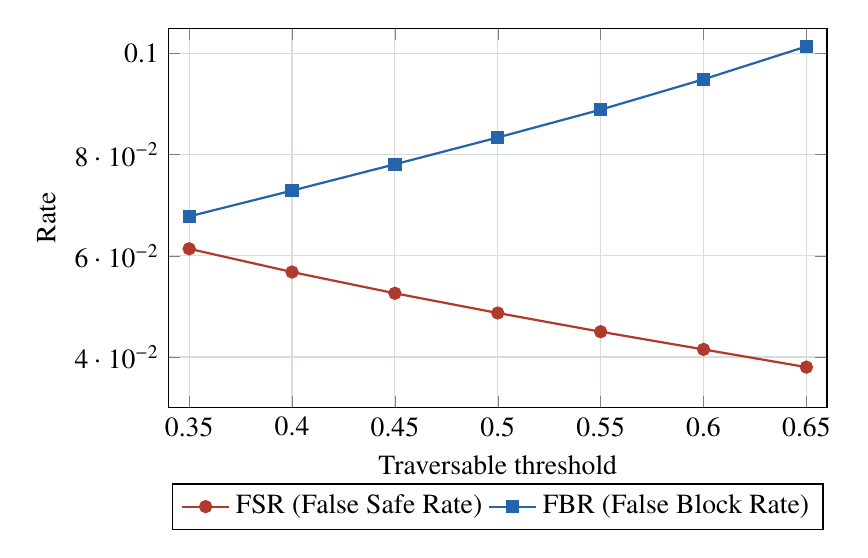
\begin{tikzpicture}
\begin{axis}[
    width=0.82\textwidth,
    height=6.4cm,
    xlabel={Traversable threshold},
    ylabel={Rate},
    ymin=0.03,
    ymax=0.105,
    xmin=0.34,
    xmax=0.66,
    grid=both,
    grid style={line},
    legend style={at={(0.5,-0.20)},anchor=north,legend columns=2},
]
\addplot[color=safety,mark=*,thick] coordinates {
  (0.35,0.0614) (0.40,0.0568) (0.45,0.0526) (0.50,0.0487) (0.55,0.0450) (0.60,0.0415) (0.65,0.0380)
};
\addlegendentry{FSR (False Safe Rate)}
\addplot[color=block,mark=square*,thick] coordinates {
  (0.35,0.0678) (0.40,0.0729) (0.45,0.0781) (0.50,0.0834) (0.55,0.0889) (0.60,0.0949) (0.65,0.1014)
};
\addlegendentry{FBR (False Block Rate)}
\end{axis}
\end{tikzpicture}
\captionof{figure}{Safety--conservativeness trade-off as a function of traversable threshold.}
\label{fig:threshold_sweep}
\end{center}

The optimal mIoU threshold is 0.45.
The FSR--FBR crossover occurs near threshold 0.40.
For safety-critical deployment, a higher threshold (0.55--0.65) reduces FSR to 3.8--4.5\% at the cost of 8.9--10.1\% FBR.

\section{CPU Inference Speed}

\begin{table}[H]
\centering
\caption{CPU inference benchmark.}
\label{tab:inference}
\begin{tabular}{@{}lr@{}}
\toprule
\textbf{Item} & \textbf{Value} \\
\midrule
CPU                & AMD Ryzen 5 5500, 6c/12t \\
Device             & CPU (no GPU) \\
Batch size         & 1 \\
Images measured    & 160 forward passes \\
\textbf{FPS}       & \textbf{22.14} \\
\textbf{Mean latency} & \textbf{45.17 ms/image} \\
P50 latency        & 44.48 ms/image \\
P95 latency        & 54.01 ms/image \\
\bottomrule
\end{tabular}
\end{table}

\section{Comparison with CaT Literature}
\label{sec:comparison}

Since the CaT classes represent nested traversability levels (sedan $\subset$
pickup $\subset$ off-road), comparisons are valid only when both studies use
the same merged label definition and evaluation split. Our blue-only result can
be compared directly with the original paper's sedan IoU; the other published
label mappings require separate treatment.

\subsection{Sedan Traversability (Blue-Only Binary)}

Our blue-only experiments directly answer ``what terrain can a sedan traverse?''---the most conservative path.
The label definition of traversable IoU matches sedan per-class IoU, although
the models and training protocols remain different:

\begin{table}[H]
\centering
\caption{Sedan traversability comparison with literature.}
\label{tab:sedan_comparison}
\small
\begin{tabular}{@{}lrrl@{}}
\toprule
\textbf{Model} & \textbf{Params} & \textbf{Sedan IoU} & \textbf{Notes} \\
\midrule
PSPNet/ResNet-18~\cite{sharma2022cat}  & ${\sim}$11M & 90.44\% & 4-class, ImageNet pretrained \\
PSPNet/ResNet-34~\cite{sharma2022cat}  & ${\sim}$21M & 91.22\% & 4-class, ImageNet pretrained \\
PSPNet/ResNet-50~\cite{sharma2022cat}  & ${\sim}$26M & 90.70\% & 4-class, ImageNet pretrained \\
PSPNet/ResNet-101~\cite{sharma2022cat} & ${\sim}$43M & \textbf{91.65\%} & 4-class, ImageNet pretrained \\
EfficientViT~\cite{efficientvit_offroad} & --- & 98.22\% & \textcolor{warn}{$\triangle$ Non-independent evaluation concern (Sec. \ref{sec:cat_literature})} \\
\midrule
\textbf{Ours --- PIDNet-S} (\texttt{conservative}) & \textbf{${\sim}$7.6M} & \textbf{82.02\%} & 2-class, from scratch \\
\textbf{Ours --- ROD} (paper recipe) & 29.1M total & \textbf{89.70\%} & 2-class, frozen pretrained ViT-S \\
\bottomrule
\end{tabular}
\end{table}

ROD reduces the gap to the best clean literature sedan result
(PSPNet/ResNet-101, 91.65\%) from 9.63 points for PIDNet-S to 1.95 points.
The remaining comparison still mixes binary and four-class optimisation, but
the sedan-positive pixel definition is aligned. The gain is consistent with
pretrained transformer features being data-efficient on CaT's 1{,}002-image
training split.
The PSPNet baselines use pretrained ResNet backbones that provide strong low-level features from the outset---a significant advantage on a small dataset (1{,}002 training images).
The EfficientViT result (98.22\%) is not treated as directly comparable because the
reported protocol raises the non-independent evaluation concern documented in
Section~\ref{sec:cat_literature}. This is a limitation of comparability, not a
claim about the authors' intent.

\subsection{Pickup Traversability (Blue+Green Binary)}

Our blue+green experiments answer ``what terrain can a pickup traverse?''---combining sedan-traversable and pickup-traversable terrain into one class:

\begin{table}[H]
\centering
\caption{Pickup-level traversability results (no clean literature comparable).}
\label{tab:pickup_comparison}
\small
\begin{tabular}{@{}lrrl@{}}
\toprule
\textbf{Model} & \textbf{Params} & \textbf{Trav.\ IoU} & \textbf{Notes} \\
\midrule
\textbf{Ours --- PIDNet-S} (\texttt{augment\_off}) & ${\sim}$7.6M & \textbf{87.90\%} & Best overall \\
Ours --- PIDNet-S (\texttt{blue\_green\_best}) & ${\sim}$7.6M & 86.06\% & With augmentation \\
\textbf{Ours --- ROD} (paper recipe) & 29.1M total & \textbf{91.34\%} & Frozen pretrained ViT-S \\
\bottomrule
\end{tabular}
\end{table}

No clean literature result reports the merged sedan+pickup traversability IoU directly.
The CaT paper's per-class pickup IoU (66--69\%) measures only the green-only pixels in the 4-class setting, which captures the additional terrain a pickup can handle beyond a sedan---a different and harder metric.
Our merged blue+green IoU is not directly comparable to that number.

\subsection{Off-Road-Vehicle Traversability (Blue+Green+Red Binary)}

Ramtekkar et al.~\cite{ramtekkar2024depth} merge all three traversable CaT
classes into a single road class. This is a more permissive target than the
blue+green pickup-level mapping used for our best model:

\begin{table}[H]
\centering
\caption{Published result for merged off-road-vehicle traversability on CaT.}
\label{tab:offroad_level_comparison}
\small
\begin{tabular}{@{}lrrl@{}}
\toprule
\textbf{Model} & \textbf{Params} & \textbf{Road IoU} & \textbf{Notes} \\
\midrule
SegFormer/MiT-B3~\cite{ramtekkar2024depth} & ${\sim}$64M & 76.28\% & Blue+green+red; split unspecified \\
\bottomrule
\end{tabular}
\end{table}

The paper also reports 88.92\% precision, 85.97\% recall, and 85.42\% F1 on
CaT. Its depth-refinement contribution is evaluated qualitatively rather than
quantitatively on CaT. Because CaT is included among the public datasets used
by its training/data-generation pipeline and the exact evaluation split is not
reported, the 76.28\% result cannot be used as a controlled baseline for our
models. Moreover, this thesis has no blue+green+red experiment, so there is no
matching label definition to compare.

\subsection{Comparability Summary}

\begin{table}[H]
\centering
\caption{What is and is not comparable.}
\label{tab:comparability}
\small
\begin{tabularx}{\textwidth}{@{}Xc@{}}
\toprule
\textbf{Comparison} & \textbf{Valid?} \\
\midrule
Our blue-only trav.\ IoU vs.\ literature sedan IoU               & \textcolor{good}{\textbf{Yes}} \\
Our blue+green trav.\ IoU vs.\ literature pickup IoU (green-only) & \textcolor{safety}{\textbf{No}} \\
Our blue+green trav.\ IoU vs.\ Ramtekkar et al.\ blue+green+red IoU & \textcolor{safety}{\textbf{No}} \\
Our binary mIoU vs.\ literature 4-class mIoU                      & \textcolor{safety}{\textbf{No}} \\
Any result vs.\ EfficientViT~\cite{efficientvit_offroad}          & \textcolor{warn}{\textbf{Not controlled}} \\
\bottomrule
\end{tabularx}
\end{table}

\subsection{Contextualised Interpretation}

The original PIDNet-S sedan-comparable result (82.02\% IoU) is 9.63 points
below PSPNet/ResNet-101 (91.65\%), whereas ROD reaches 89.70\%. This accuracy
improvement changes the deployment trade-off rather than eliminating it:
\begin{enumerate}[nosep]
  \item \textbf{$5.7\times$ fewer parameters} (7.6M vs.\ 43M for ResNet-101),
  making PIDNet-S a candidate for later embedded-hardware validation.
  \item \textbf{PIDNet-S requires no pretraining}, whereas ROD's accuracy gain
  depends on the 22.35M-parameter frozen EfficientSAM encoder.
  \item \textbf{Measured CPU throughput} of 22.14~FPS on the stated Ryzen~5
  system. No hardware-matched PSPNet benchmark was performed, so the speed
  results are not used for a direct cross-paper comparison.
  \item \textbf{Safety metrics reported} (FSR 4.32\%, FBR 7.04\%)---these
  asymmetric-error metrics were not provided by the CaT baselines surveyed.
\end{enumerate}

The architecture suite shows that pretraining and global transformer context
are a successful route toward closing the clean-literature accuracy gap, but
does not isolate pretraining from architecture because both change together.

\section{Qualitative Results}

To provide intuition for the model's performance, we visualise successful test
examples in Figure~\ref{fig:qualitative_cat}, ranked failure modes in
Figure~\ref{fig:qualitative_failures}, and unscored model behaviour on ALICE
platform data in Figure~\ref{fig:qualitative_alice}.

\begin{figure}[H]
\centering
\includegraphics[width=0.48\linewidth]{../outputs/controlled_ablation_augment_off/test_top_success/best_triptychs/mixed_pln_1311.png}
\hfill

\includegraphics[width=0.48\linewidth]{../outputs/controlled_ablation_augment_off/test_top_success/best_triptychs/mixed_pln_1306.png}

\vspace{0.2cm}

\includegraphics[width=0.48\linewidth]{../outputs/controlled_ablation_augment_off/test_top_success/best_triptychs/mixed_pln_1188.png}
\hfill

\includegraphics[width=0.48\linewidth]{../outputs/controlled_ablation_augment_off/test_top_success/best_triptychs/mixed_pln_1282.png}
\caption{High-performing qualitative results on the CaT test set, selected by
lowest per-image sum of false-safe and false-block rates. Each triptych shows
the RGB input (left), binary ground truth (centre), and PIDNet-S prediction
(right). These examples document successful cases and are not presented as
failure cases; the selection rule and image identifiers make the panel
reproducible.}
\label{fig:qualitative_cat}
\end{figure}

\begin{figure}[H]
\centering

\includegraphics[width=0.32\linewidth]{../outputs/controlled_ablation_augment_off/test_review/worst_false_safe/mixed_pln_1278.png}
\hfill

\includegraphics[width=0.32\linewidth]{../outputs/controlled_ablation_augment_off/test_review/worst_false_block/mixed_425.png}
\hfill

\includegraphics[width=0.32\linewidth]{../outputs/controlled_ablation_augment_off/test_review/worst_boundary_error/mixed_459.png}
\caption{Safety-oriented CaT failure cases selected from all 544 test images.
Each triptych shows RGB input, ground truth, and prediction from left to right;
green denotes traversable and red untraversable. Left:
\texttt{mixed\_pln\_1278}, the highest per-image false-safe rate
(FSR 30.20\%, FBR 0.19\%). Centre: \texttt{mixed\_425}, the highest
false-block rate (FBR 52.84\%, FSR 0.67\%). Right: \texttt{mixed\_459}, a
boundary-error example (49.72\% error within a four-pixel-wide ground-truth
boundary band; FSR 5.63\%, FBR 10.70\%). Selection and metrics were computed
at the frozen 0.50 threshold by \texttt{ttfm.cli review}.}
\label{fig:qualitative_failures}
\end{figure}

Figure~\ref{fig:qualitative_failures} exposes complementary risks hidden by
the aggregate mIoU. In the false-safe example, visually similar pale field and
track surfaces cause the predicted traversable region to expand far beyond the
annotated corridor. In the false-block example, the model retains only a small
part of a narrow, shadowed trail, producing conservative loss of usable space.
The third example shows lateral disagreement along an irregular vegetation--path
interface. Boundary error is defined here as the fraction of misclassified
pixels inside a band formed by dilating and eroding the ground-truth boundary
by two pixels. These cases are deliberately selected extremes and therefore
characterise failure modes rather than typical test performance.

\begin{figure}[H]
\centering
\includegraphics[width=0.48\linewidth]{../outputs/alice_preview/triptychs/alice_scenario02_sequence01_0000_1697206492496274000_camera_left.png}
\hfill
\includegraphics[width=0.48\linewidth]{../outputs/alice_preview/triptychs/alice_scenario02_sequence02_0005_1697207730943946000_camera_left.png}

\vspace{0.2cm}
\includegraphics[width=0.48\linewidth]{../outputs/alice_preview/triptychs/alice_scenario02_sequence04_0002_1697208533728029000_camera_left.png}
\hfill
\includegraphics[width=0.48\linewidth]{../outputs/alice_preview/triptychs/alice_scenario02_sequence05_0009_1697208974627527000_camera_left.png}
\caption{Unscored qualitative transfer examples on unlabelled ALICE data. Each
triptych shows the RGB input (left), prediction overlay (centre), and binary
prediction (right). ALICE was not used for training and has no ground truth in
this study; consequently, the panel illustrates model behaviour under a camera
and environment shift but does not establish cross-dataset accuracy.}
\label{fig:qualitative_alice}
\end{figure}


% ============================================================
\chapter{Discussion}
\label{sec:discussion}
% ============================================================

\section{Key Findings}

\textbf{ROD's advantage is reproducible rather than a favourable seed.}
Across three matched seeds, the standard deviation of mIoU is at most 0.0010
for ROD, while its mean advantage over PIDNet-S is 0.0315--0.0379 depending on
the label policy. ROD also reduces both false-safe and false-block rates, which
rules out a simple operating-point shift as the explanation.

\textbf{The documented ROD recipe transfers better than the original CaT recipe.}
Cross-entropy alone, neutral class weights, batch size 8, learning rate
$10^{-3}$, and iteration-level polynomial decay produce the strongest models
in the study. This reverses the PIDNet ablation's local conclusion that biased
class weights plus CE+Dice are the preferred default; optimisation conclusions
are architecture-dependent.

\textbf{Accuracy and latency select different winners.}
ROD gives the best accuracy and safety metrics, but PIDNet-S is 12.5 times
faster in the controlled H100 FP32 benchmark. A deployment decision must
therefore specify both a safety/accuracy target and a latency budget.

\textbf{Augmentation hurts on this dataset.}
The most surprising result is that disabling augmentation improved all metrics: mIoU rose from 0.8667 to 0.8939, FSR dropped from 5.89\% to 4.32\%, and FBR dropped from 8.48\% to 7.04\%.
This 2.7 percentage point mIoU improvement from a single-factor change is the largest effect in the ablation study.

One plausible explanation is that the current augmentation recipe (colour
jitter, blur, and sharpness) introduces changes that do not match useful
variation in the CaT training distribution. The ablation establishes the
effect for this recipe and run, but does not determine the mechanism or imply
that augmentation is generally harmful.

\textbf{Blue+green mapping produced the best observed result.}
The transition from blue-only to blue+green traversable labels improved mIoU from 0.8374 (5-epoch baseline) to 0.8780 (15-epoch blue+green).
Because this comparison is confounded by epoch budget and target definition,
it does not isolate a causal benefit of the mapping. It shows only that the
blue+green operating definition produced the strongest observed result in the
experiments performed.

\textbf{False-safe penalty loss is counterproductive.}
The false-safe penalty worsened all metrics, including FSR itself (7.45\% vs.\ 5.89\% baseline).
This penalty effectively pushes the model's decision boundary uniformly, including in regions where the model was already correct.
The threshold sweep provides a more principled and effective way to tune the safety--conservativeness trade-off post-hoc.

\textbf{Higher resolution does not help.}
Increasing resolution from $640\times384$ to $720\times448$ slightly reduced mIoU (0.8632 vs.\ 0.8667) and increased FBR (9.28\% vs.\ 8.48\%).
The CaT images have sufficient detail at $640\times384$ for binary traversability, and the higher resolution reduced the effective batch size from 4 to 2, potentially degrading gradient estimation quality.

\textbf{Class weight tuning matters but is secondary.}
Neutral weights $[1.0, 1.0]$ performed well (0.8848 mIoU, lowest FBR at 6.95\%), suggesting that the computed inverse-frequency weights with bias may not be optimal.
However, the difference from the baseline is smaller than the augmentation effect.

\section{Limitations}

\begin{enumerate}[nosep]
  \item \textbf{Small dataset}: 1{,}002 training images from only three trail environments limits the model's ability to generalise to diverse off-road conditions.
  \item \textbf{Pretraining is confounded with architecture}: PIDNet-S was
  trained from scratch while ROD uses EfficientSAM pretraining. The experiments
  establish an end-to-end model-family difference, not the isolated causal
  contribution of pretraining.
  \item \textbf{No automotive embedded platform}: GPU speed is measured on an
  H100 MIG partition and a local desktop RTX~5060, not a Jetson or production
  vehicle computer. Power, thermals, camera capture, and planner integration
  remain outside scope.
  \item \textbf{No cross-dataset evaluation}: The model was not evaluated on RUGD, RELLIS-3D, or other off-road datasets.
  \item \textbf{Limited augmentation exploration}: Only one augmentation recipe was tested. Geometric augmentations (rotation, scale, crop) and more domain-specific augmentations (weather, lighting variation) were not explored.
\end{enumerate}

\section{Practical Deployment Considerations}

The 22~FPS PIDNet-S CPU throughput at $640\times384$ suggests that deployment
on a mobile robot with a mid-range CPU is feasible for low-speed navigation.
ROD instead requires GPU acceleration in its present form because every frame
passes through the full $1024\times1024$ ViT encoder. Even on the H100 MIG
partition, eager FP32 ROD reaches only 21.8~FPS compared with 272~FPS for
PIDNet-S. The RTX~5060 edge-style experiment in
Section~\ref{sec:edge_benchmark} measures reduced-precision batch-1 operation
including the deployment-relevant processing stages defined there.

The 4.32\% FSR means that roughly 1 in 23 untraversable pixels is misclassified as safe.
In practice, these errors tend to cluster at class boundaries (edges of obstacles, vegetation borders), so the effective safety risk depends on the downstream planner's spatial aggregation.
A planner that inflates obstacles or requires contiguous traversable regions would be more robust to scattered false-safe pixels.


% ============================================================
\chapter{Conclusions}
\label{sec:conclusions}
% ============================================================

This thesis presented a complete pipeline for binary traversability segmentation
on CaT and compared a lightweight real-time CNN (PIDNet-S) with a frozen
pretrained transformer architecture (ROD).
The main conclusions are:

\begin{enumerate}
  \item \textbf{ROD reproducibly outperforms PIDNet-S}: mean mIoU improves
  from 88.22\% to 91.38\% for blue+green and from 88.32\% to 92.11\% for
  blue-only over three matched seeds.

  \item \textbf{The closest documented ROD recipe is strongest}: it reaches
  92.36\% mIoU for blue+green and 92.80\% for blue-only, while reducing both
  false-safe and false-block errors relative to the matched PIDNet means.

  \item \textbf{The accuracy gain has a large latency cost, which can be mitigated}: on the same H100
  MIG partition, eager FP32 batch-1 ROD is 12.5 times slower than PIDNet-S
  (45.86 vs. 3.67~ms). This prevents treating the paper's A6000 speed claim as
  directly portable to edge hardware. However, on the local RTX~5060, compiling the models with TensorRT FP16 (with mixed-precision fallbacks) successfully mitigates this cost: the pipeline latency drops to 25.39~ms, enabling ROD to run at 39.4~FPS and cross the critical 30~FPS real-time threshold.

  \item \textbf{Controlled ablation reveals} that, under the tested settings,
  disabling the augmentation recipe improves all reported metrics, the tested
  false-safe penalty is counterproductive, and the tested higher resolution
  does not improve accuracy.

  \item \textbf{ROD substantially closes the sedan-IoU literature gap}:
  blue-only traversable IoU rises from 82.02\% for the original PIDNet run to
  89.70\%, versus 91.65\% for PSPNet/ResNet-101 under a different four-class
  training protocol.
\end{enumerate}


% ============================================================
\chapter{Future Work}
\label{sec:future}
% ============================================================

\section{Plan to Completion --- July 2026}
\label{sec:july_plan}

The remaining thesis period runs from 10 to 31 July 2026. The priority is to
deliver a verified and clearly documented thesis based on the current best
model, rather than destabilising the results with a broad final round of model
development.

\begin{table}[H]
\centering
\caption{Dated completion plan for the remainder of July 2026.}
\label{tab:july_plan}
\small
\begin{tabularx}{\textwidth}{@{}p{2.1cm}p{2.0cm}X@{}}
\toprule
\textbf{Dates} & \textbf{Priority} & \textbf{Actions and exit criterion} \\
\midrule
10--12 July & Complete & Freeze the PIDNet-S baseline, integrate ROD, and
verify the three-seed architecture suite against saved evaluation artifacts. \\

13--17 July & Required & Add representative CaT successes, boundary errors,
and failure cases, plus a small ALICE out-of-distribution panel. Complete
captions, provenance, and interpretation for every figure. \\

18--21 July & Complete & Matched RTX~5060 edge-style benchmark completed with
FP16 accuracy verification, latency distributions, and peak-memory reporting. \\

22--24 July & Required & Perform a full technical edit: reconcile terminology,
cross-references, tables, citations, limitations, and conclusions. Produce and
send a supervisor-review PDF by 24 July. \\

25--27 July & Required & Incorporate supervisor feedback received in the review
window, resolve all remaining placeholders, and complete the bibliography and
appendices. \\

28--29 July & Required & Apply final UC3M cover assets and PDF/A metadata;
rebuild contents and lists; check links, page numbering, figure sources,
spelling, and academic-integrity requirements. \\

30--31 July & Buffer & Create the final submission artifact and submit on 30
July if possible. Reserve 31 July only for compilation, upload, or approval
problems. \\
\bottomrule
\end{tabularx}
\end{table}

\noindent\textbf{Experiment stop rule.}
The architecture and multi-seed training campaign is complete. No new training
begins after this suite; remaining experiments are deployment benchmarks or
post-hoc analyses of saved checkpoints.

\section{Short-term (Remaining Thesis Period)}
\begin{itemize}[nosep]
  \item \textbf{Reproducibility of the verified baseline}: The portable frozen
  configuration is \texttt{configs/frozen\_pidnet\_cat.yaml}. The best
  checkpoint is \texttt{outputs/controlled\_ablation\_augment\_off/checkpoints/best.pt};
  evaluation uses \texttt{ttfm.cli eval}. Artifact hashes and expected output
  are recorded in \texttt{reports/reproducibility\_baseline.md}.
  \item \textbf{Qualitative evidence completed}: Figures~\ref{fig:qualitative_cat}--\ref{fig:qualitative_alice}
  include ranked CaT successes, false-safe, false-block, and boundary-error
  cases, plus explicitly unscored ALICE examples.
  \item \textbf{Edge-style measurement completed}: both saved model families
  were benchmarked on the same RTX~5060 with batch size 1, FP16 weights,
  postprocessing, synchronisation, and peak-memory reporting.
  \item \textbf{Finish the document}: prioritize supervisor feedback,
  references, figure provenance, UC3M formatting, proofreading, and a validated
  final PDF over optional experiments.
\end{itemize}

\section{Medium-term Extensions}
\begin{itemize}[nosep]
  \item \textbf{Isolate pretraining from architecture}: compare pretrained and
  from-scratch encoders within one model family.
  \item \textbf{Expanded augmentation ablation}: separate geometric,
  photometric, and domain-specific augmentation effects.
  \item \textbf{ONNX/TensorRT export}: optimise the saved model and benchmark
  end-to-end latency on representative embedded hardware.
  \item \textbf{4-class CaT segmentation}: Extend the pipeline to the full 4-class task for direct comparison with CaT baselines.
  \item \textbf{Cross-dataset evaluation}: Evaluate on RUGD and RELLIS-3D to assess generalisation.
  \item \textbf{Self-supervised and semi-supervised methods}: Leverage unlabelled frames (e.g., from ALICE robot sequences) through self-training or contrastive learning.
  \item \textbf{Temporal consistency}: Exploit video sequences for temporally coherent predictions using optical flow or recurrent architectures.
\end{itemize}

\section{Long-term Research Directions}
\begin{itemize}[nosep]
  \item \textbf{Multi-sensor fusion}: Combine RGB segmentation with LiDAR or depth for robust traversability in challenging lighting and weather.
  \item \textbf{Uncertainty estimation}: Produce calibrated uncertainty maps alongside traversability masks to inform risk-aware planning.
  \item \textbf{Online adaptation}: Adapt the model online using self-supervised traversability signals from the robot's own driving experience.
\end{itemize}

% ============================================================
% REFERENCES
% ============================================================
\clearpage
\phantomsection
\addcontentsline{toc}{chapter}{Bibliography}
\bibliographystyle{IEEEtranN}
% Inline bibliography since .bib file may not exist yet.
\begin{thebibliography}{12}

\bibitem[Sharma et~al.(2022)]{sharma2022cat}
S.~Sharma, J.~E. Ball, B.~Tang, D.~W. Carruth, M.~Doude, and M.~A. Islam.
\newblock CaT: CAVS Traversability Dataset for Off-Road Autonomous Driving.
\newblock \emph{IEEE Access}, 10:24759--24768, 2022.

\bibitem[Xu et~al.(2023)]{xu2023pidnet}
J.~Xu, Z.~Xiong, and S.~P. Bhattacharyya.
\newblock PIDNet: A Real-time Semantic Segmentation Network Inspired by PID Controllers.
\newblock In \emph{Proceedings of the IEEE/CVF Conference on Computer Vision and Pattern Recognition (CVPR)}, pages 19529--19539, 2023.

\bibitem[Faykus et~al.(2024)]{efficientvit_offroad}
M.~H.~Faykus~III, A.~Pickeral, E.~Marquez, M.~C.~Smith, and J.~C.~Calhoun.
\newblock Efficient Vision Transformers for Autonomous Off-Road Perception Systems.
\newblock \emph{Journal of Computer and Communications}, 12(9):188--207, 2024.
\newblock \url{https://doi.org/10.4236/jcc.2024.129011}.

\bibitem[Ramtekkar et~al.(2024)]{ramtekkar2024depth}
V.~V. Ramtekkar, L.~Dahiya, N.~Shah, K.~Nishimiya, T.~Kuroki,
C.~Song, A.~Kim, and M.-H.~Jeon.
\newblock Robust Depth-Aided Segmentation for Drivable Region Detection in
Challenging Environments.
\newblock In \emph{ICRA 2024 Workshop on Resilient Off-road Autonomy}, poster,
2024.
\newblock \url{https://openreview.net/forum?id=qzVdN0ZRt9}.

\bibitem[Wigness et~al.(2019)]{wigness2019rugd}
M.~Wigness, S.~Eum, J.~G. Rogers~III, D.~Han, and H.~Kwon.
\newblock A RUGD Dataset for Autonomous Navigation and Visual Perception in Unstructured Outdoor Environments.
\newblock In \emph{International Conference on Intelligent Robots and Systems (IROS)}, 2019.

\bibitem[Jiang et~al.(2021)]{jiang2021rellis}
P.~Jiang, P.~Osteen, M.~Wigness, and S.~Saripalli.
\newblock RELLIS-3D Dataset: Data, Benchmarks and Analysis for Off-Road Robotics.
\newblock In \emph{IEEE International Conference on Robotics and Automation (ICRA)}, 2021.

\bibitem[Triest et~al.(2022)]{triest2022tartandrive}
S.~Triest, M.~Sivaprakasam, S.~J. Wang, W.~Wang, A.~M. Johnson, and S.~Scherer.
\newblock TartanDrive: A Large-Scale Dataset for Learning Off-Road Dynamics Models.
\newblock In \emph{IEEE International Conference on Robotics and Automation (ICRA)}, 2022.
\newblock doi:10.1109/ICRA46639.2022.9811648.

\bibitem[Min et~al.(2022)]{min2022orfd}
C.~Min, W.~Jiang, D.~Zhao, J.~Xu, L.~Xiao, Y.~Nie, and B.~Dai.
\newblock ORFD: A Dataset and Benchmark for Off-Road Freespace Detection.
\newblock \emph{arXiv preprint arXiv:2206.09907}, 2022.

\bibitem[Zhao et~al.(2017)]{zhao2017pspnet}
H.~Zhao, J.~Shi, X.~Qi, X.~Wang, and J.~Jia.
\newblock Pyramid Scene Parsing Network.
\newblock In \emph{Proceedings of the IEEE Conference on Computer Vision and Pattern Recognition (CVPR)}, pages 2881--2890, 2017.

\bibitem[He et~al.(2016)]{he2016resnet}
K.~He, X.~Zhang, S.~Ren, and J.~Sun.
\newblock Deep Residual Learning for Image Recognition.
\newblock In \emph{Proceedings of the IEEE Conference on Computer Vision and Pattern Recognition (CVPR)}, pages 770--778, 2016.

\bibitem[Sun et~al.(2025)]{sun2025rod}
T.~Sun, H.~Ye, J.~Mei, L.~Chen, F.~Zhao, L.~Zong, and Y.~Hu.
\newblock ROD: RGB-Only Fast and Efficient Off-road Freespace Detection.
\newblock \emph{arXiv preprint arXiv:2508.08697}, 2025.

\bibitem[Xiong et~al.(2024)]{xiong2024efficientsam}
Y.~Xiong, B.~Varadarajan, L.~Wu, X.~Xiang, F.~Xiao, C.~Zhu, X.~Dai,
D.~Wang, F.~Sun, and F.~Iandola.
\newblock EfficientSAM: Leveraged Masked Image Pretraining for Efficient
Segment Anything.
\newblock In \emph{Proceedings of the IEEE/CVF Conference on Computer Vision
and Pattern Recognition (CVPR)}, 2024.

\end{thebibliography}


% ============================================================
% APPENDICES
% ============================================================
\appendix
\chapter{Full Configuration Reference --- PIDNet Ablation Best}
\label{app:config}

\begin{verbatim}
seed: 1337
processed_root: data_processed_blue_green
dataset_name: mixed
experiment_name: controlled_ablation_augment_off
preprocessing:
  val_fraction: 0.2
  traversable_palette_names: [blue, green]
training:
  model_name: pidnet-s
  input_size: [640, 384]
  batch_size: 4
  epochs: 15
  learning_rate: 0.00025
  min_learning_rate: 0.00001
  weight_decay: 0.0001
  mixed_precision: bf16
  augment: false
  untraversable_weight_bias: 2.5
  traversable_weight_bias: 0.75
postprocessing:
  traversable_threshold: 0.5
\end{verbatim}

\section*{ROD Paper-Recipe Configuration}

\begin{verbatim}
seed: 1337
processed_root: data_processed_blue_green
experiment_name: mixed_binary_traversability_rod_vits_paper
training:
  model_name: rod-vits
  rod_encoder_checkpoint: weights/efficient_sam_vits.pt
  rod_encoder_image_size: 1024
  input_size: [640, 384]
  batch_size: 8
  val_batch_size: 4
  epochs: 15
  learning_rate: 0.001
  weight_decay: 0.01
  lr_scheduler: poly
  poly_power: 0.9
  mixed_precision: bf16
  augment: false
  class_weights: [1.0, 1.0]
  ce_loss_weight: 1.0
  dice_loss_weight: 0.0
postprocessing:
  traversable_threshold: 0.5
\end{verbatim}


\chapter{Dataset Split Summary}
\label{app:splits}

\begin{table}[H]
\centering
\caption{Dataset split by trail environment.}
\begin{tabular}{@{}lrrrr@{}}
\toprule
\textbf{Subset} & \textbf{Train} & \textbf{Val} & \textbf{Test} & \textbf{Total} \\
\midrule
Brown Field  & ${\sim}$140 & ${\sim}$35  & 60  & ${\sim}$235 \\
Main Trail   & ${\sim}$133 & ${\sim}$33  & 57  & ${\sim}$223 \\
Power Line   & ${\sim}$729 & ${\sim}$198 & 427 & ${\sim}$1{,}354 \\
\midrule
\textbf{Mixed total} & \textbf{1{,}002} & \textbf{266} & \textbf{544} & \textbf{1{,}812} \\
\bottomrule
\end{tabular}
\end{table}


\chapter{CaT Original 4-Class Benchmark}
\label{app:cat_benchmark}

From the dataset file \texttt{CAT/mixed/test\_result\_info}:

\begin{table}[H]
\centering
\caption{CaT original 4-class results (PSPNet, from dataset distribution).}
\label{tab:cat_original}
\small
\begin{tabular}{@{}ll rrrr rrrr@{}}
\toprule
\textbf{Network} & \textbf{Backbone} & \textbf{OA} & \textbf{MA} & \textbf{FWA} & \textbf{mIoU} & \textbf{BG} & \textbf{Sedan} & \textbf{Pickup} & \textbf{Off-road} \\
\midrule
PSPNet & ResNet-18  & 92.78 & 90.41 & 87.11 & 82.84 & 94.60 & 90.44 & 66.62 & 79.71 \\
PSPNet & ResNet-34  & 93.20 & 91.06 & 87.78 & 83.79 & 94.79 & 91.22 & 68.65 & 80.52 \\
PSPNet & ResNet-50  & 92.93 & 90.60 & 87.34 & 83.18 & 94.63 & 90.70 & 67.40 & 80.00 \\
PSPNet & ResNet-101 & 93.42 & 91.24 & 88.12 & 84.18 & 95.00 & 91.65 & 69.08 & 81.00 \\
\bottomrule
\end{tabular}
\end{table}


\chapter{All Run Configurations Summary}
\label{app:all_configs}

\begin{table}[H]
\centering
\caption{Complete configuration for all experimental runs.}
\label{tab:all_configs}
\scriptsize
\begin{tabular}{@{}lcrcclcrr@{}}
\toprule
\textbf{Run} & \textbf{Res.} & \textbf{Ep.} & \textbf{LR} & \textbf{Aug.} & \textbf{Trav.\ map} & \textbf{Wt.\ bias} & \textbf{FS pen.} & \textbf{Thr.} \\
\midrule
\texttt{default}       & $640\times384$ & 5  & $3\!\times\!10^{-4}$   & Yes & Blue only & --- & 0.0  & 0.50 \\
\texttt{conservative}  & $640\times384$ & 15 & $2.5\!\times\!10^{-4}$ & Yes & Blue only & 2.5/0.75 & 0.0  & 0.50 \\
\texttt{third\_run}    & $720\times448$ & 18 & $2\!\times\!10^{-4}$   & Yes & Blue only & 2.5/0.75 & 0.35 & 0.58 \\
\texttt{fourth\_run}   & $720\times448$ & 18 & $2.2\!\times\!10^{-4}$ & Yes & Blue only & 2.5/0.75 & 0.0  & 0.53 \\
\texttt{blue\_green}   & $640\times384$ & 15 & $2.5\!\times\!10^{-4}$ & Yes & B+G       & 2.5/0.75 & 0.0  & 0.50 \\
\midrule
\texttt{abl\_baseline} & $640\times384$ & 15 & $2.5\!\times\!10^{-4}$ & Yes & B+G       & 2.5/0.75 & 0.0  & 0.50 \\
\texttt{abl\_loss\_fs}  & $640\times384$ & 15 & $2.5\!\times\!10^{-4}$ & Yes & B+G       & 2.5/0.75 & 0.35 & 0.50 \\
\texttt{abl\_aug\_off} & $640\times384$ & 15 & $2.5\!\times\!10^{-4}$ & \textbf{No} & B+G  & 2.5/0.75 & 0.0  & 0.50 \\
\texttt{abl\_720}      & $720\times448$ & 15 & $2.5\!\times\!10^{-4}$ & Yes & B+G       & 2.5/0.75 & 0.0  & 0.50 \\
\texttt{abl\_neutral}  & $640\times384$ & 15 & $2.5\!\times\!10^{-4}$ & Yes & B+G       & 1.0/1.0  & 0.0  & 0.50 \\
\midrule
\texttt{rod\_controlled} & $640\times384$ & 15 & $2.5\!\times\!10^{-4}$ & Yes & Both policies & 2.5/0.75 & 0.0 & 0.50 \\
\texttt{pid/rod\_seeds} & $640\times384$ & 15 & $2.5\!\times\!10^{-4}$ & Yes & Both policies & 2.5/0.75 & 0.0 & 0.50 \\
\texttt{rod\_paper} & $640\times384$ & 15 & $1\!\times\!10^{-3}$ & No & Both policies & 1.0/1.0 & 0.0 & 0.50 \\
\bottomrule
\end{tabular}
\end{table}


\end{document}
